\chapter{Requirements Analysis}
\label{chapter:requirements-analysis}
Based on the fundamentals the requirements for the protoype to be developed will be formulated in this chapter.
Thereby relevant aspects for the specific implementation will be considered.
The analysis, the creation of requirments and the commitment from all sides to these requirements is an important step to sucessfully realize a project, not only in the software development area.
It does not matter if it is a private project, a company product or a project from a customer.
The better a project is defined and everyone is on the same state, the better the final result will be.
In these thesis the \ac{FOKUS} acts as the customer.
Each step has to be discussed and approved by a representative of the \ac{FOKUS}.
Due to the fact that the prototype will be created from scretch most of the concepts have to be created in brainstroming meetings.
An agile development process will be used to react to rapidly changing requirements.
As mentioned before a Kanban like method will be used in this project.


\section{Technical requirements}
\label{section:technical-requirements}
% virtualization
As the fundamental requirement, the prototype to be developed has to create, manage and maintain virtualized containers on a fog node.
Tools like Open Baton inherently supports OpenStack as the \ac{ETSI} \ac{MANO} \ac{VIM} layer.
Most \ac{MANO} tools like Open Baton uses OpenStack which deploys virtual machines to virtualize the \acp{NF}.
This is a rock solid solution for a cloud environment.
Unfortunately a bare-metal virtualization is most of the times not feasible on small power devices like they are used in the \ac{IoT} area.
Therefore a much more efficient and lightweight solution like container virtualization should be used and handled by an orchestration engine.
The desired service like a \acp{NF} can be bundeled in one or multiple containers and executed afterwards on the expected \ac{IoT} nodes.
Such a bundle of containers should be passed to the node as a build plan or a blueprint of the service.
The fog node engine should accept the blueprint and deploy the containers to the desired virtualization layer.
Afterwards the lifecylce of the services should be monitored.

% constraints
The second functional requirement is the implementation of a constraint logic which will be used to filter relevant nodes during the orchestration.
A constraint can be a functional and non-functional capability.
For example a specific hardware component, like a sensor or a ZigBee dongle, which is necessary to execute the \ac{NF} or a hardware requirement, like \ac{CPU} power, \ac{RAM} or disk space.
It could also be a non-functional constraint, for example a specific software which has to be installed or a protocal which can be used.
The engine should be able to manage these constraints by itself and if necessary for all adjacent nodes and should consider them while choosing a suitable nodes for the desired \ac{NF}.
The whole functionality should work similar to the labels in Docker Swarm.
There a Docker Swarm node can be have multiple labels, which can be considered when deploying an image.
This behavior should be achieved by the fog node engine.

Another important aspect is the lifecycle management of the node, the deployed services and images.
In the prototype it has to be elaborated how the lifecycle of the several componants can be implemented.
An sample implementation of a node management lifecycle is shown in the OpenFog Reference Architecture for Fog Computing\autocite[p. 52]{OpenFog:2017}.
Figure \ref{fig:open_fog_node_mgm_lifecycle} describes the five steps of a typical lifecycle based on these architecture.
\begin{figure}[H]
    \centering
    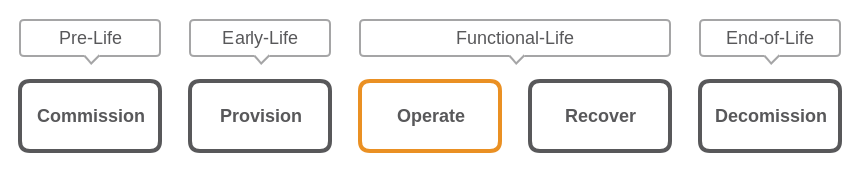
\includegraphics[width=\textwidth]{resources/images/node_management_lifecycle.png}
    \caption[Node management lifecycle]{Node management lifecycle. Adapted from: \autocite[p. 52]{OpenFog:2017}}
    \label{fig:open_fog_node_mgm_lifecycle}
\end{figure}

\begin{itemize}
  \item The \textbf{Commission} is the earliest phase in a lifecylce mostly used to perform action like identification, certificates or calibration of time.\autocite[p. 52]{OpenFog:2017}
  \item In the \textbf{Provision} phase the node will be enrolled to the system so that the node can be discovered and identified and also advertise features and capabilities.\autocite[p. 52]{OpenFog:2017}
  \item The \textbf{Operate} phase is the state of the node when everything operates normal. This includes the reliability, availability and serviceability of the node.\autocite[p. 52]{OpenFog:2017}
  \item In contrast to that the \textbf{Recover} phase performs action if something operates out of norm.\autocite[p. 52]{OpenFog:2017} The node should be able to recover to the normal state.\autocite[p. 52]{OpenFog:2017}
  \item Finally the \textbf{Decomission} phase is used for cleaning up sensitive data on the node and to unregister from other components.
\end{itemize}

In addition to the node lifecycle, an exemplarily lifecycle for services and images is shown in the \ac{ETSI} \ac{MANO} specification\autocite[p. 67 ff.]{ETSI:MANO:2014}
These lifecylce is much more detailed than the node OpenFog node lifecycle and it handles several state from the instantiation of a service, over quering some data, up to the termination of service.
Some of the specifications are tightly coupled to \acp{NFV}.
However these lifecycle specification is a good starting point to elaborate a custom solution.

Some secondary conditions should also be fulfilled.
The whole system should be modular and easy to extend.
Modules should be as decoupled as possible and the whole system should be controled via an \ac{API}.
The centralized cloud environment should be easiely replacable and should not be exclusively bound to Open Baton or any other tool.
The same applies to the prototype, it should not be bound to Docker only and should be able to use other virtualization tools.
Finally the whole system should be well tested and documented.


\section{Functional requirements}
\label{section:functional-requirements}
% prototype behavior
After the general conditions for the prototype has been defined, the functional requirements will also be addressed.
% When selecting the programming environment special attention is paid to the compatibility of the Open Baton framework. % TODO: was noch?
% This is particularly important as the effort to develop a prototype should be a s small as possible and the prototype should be natively applicable on the fog nodes.
% Open Baton has an build in plugin mechanism, which allows to replace for example the \ac{VIM} driver or the \ac{VNFM} so that any third party tool can be accessed via an \ac{API}.
% Because Open Baton and the whole environment around them is open source, it would be also feasible to extend the system if necessary, but with the addition, that the system still follows the \ac{ETSI} \ac{MANO} conventions.
% Beside that the prototype should be flexible enough to also fit in any other system by providing an \ac{API} to control the system.
% \todo{Rework that section}
%
% % GUI beahvior
% Additional it would be useful to create a \ac{GUI} for interacting with the prototype and show the functionallity of the system.
% This should only be a simple \ac{GUI} for testing and demonstration purposes and should not be necessary for executing the final prototype.
% Later on the prototype should be controlled via the \ac{API} from any other existing orchestration tool.
% A command line tool to control the system would be useful as well and eases the handling of the prototype.
\todo{Rework that section}
\todo{also more}
% TODO: probably more?

\section{Use-Case-Analysis}
\label{section:use-case-analysis}
\doit
% Deploy VNFs in factory (e.g. mass production, tracking of stuff)
% ad hoc deployment if truck arives at factory
% detect the right nodes, e.g. software needs specific sensor or latency
% Sequenzdiagramm für Ablauf vom Deployment bis zum container: IMG_20170526_201659.jpg

\section{Delineation from existing solutions}
\label{section:delineation-from-existing-solutions}
This section is intended to show the features of existing systems and the main differences will be highlighted.
As mentioned before, the prototype to be developed should orchestrate virtualized containers on nodes based on functional and non-functional constraints.
Therefore the focus of this consideration is the orchestration as well as the constraints.

\paragraph{Kubernetes} is especially made for Docker and can orchestrate, scale and manage containers.
It is open source, made by Google and one of the most popular orchestration tools out there.
It has on huge and pretty active community and is used by several well known companies\autocite{Kubernetes:Case-Studies} like ebay\footnote{\url{http://www.ebay.com}} and Wikimedia\footnote{\url{https://www.wikimedia.org}}.
Due to the fact, that is exclusivly made for Docker, it means that the system is not made to easily switch the underlying container engine if needed.

As mentioned in section \ref{subsection:state-of-the-art:kubernetes} Kubernetes supports labels.
These are simple key-value pairs provided as \ac{JSON} objects which can be added by the system administrator to a Kubernetes Object like a pod or a service.
The labels are stored on the Kubernetes Master and can be used to filter specific pods or services during the deployment phase.
This behavior is pretty close to the one which should be achieved.

Kubernetes is made for the cloud, which means it is not inteded to be used on low power devices.
There are some trials to do so, but until know it is not used in a productive \ac{IoT} environment.
Forthermore Kuberenetes is not \ac{ETSI} \ac{MANO} compliant, but provides an easy to use web \ac{UI}.

\paragraph{Docker Swarm} is pretty similar to Kubernetes from a functional point of view, which means it has nearly the same pros and cons.
It is open source as well, has a quite active community and it is also made exclusivly for Docker.
Biggest benefit compared to Kubernetes is, that it is build the Docker Engine.
No separate installation is necessary and it can be used out of the box.

Also in terms of labels, both platforms are similar.
Docker Swarm uses labels in the same way Kubernetes is using them.
The user can add them during the initialization phase or edit them during runtime.
They are also key-value pairs or alternatively keys only.
By default labels can not be predefined in a \ac{JSON} file and applied to the node afterwards.
The placement have to be done by hand via the Docker client or the \ac{REST} \ac{API}.

Just as Kubernetes, Docker Swarm is not \ac{ETSI} \ac{MANO} compliant and provides no build-in \ac{GUI}, but there are several third party tools out in the market.
Due to the fact that it is a build-in function of Docker, the setup is quite easy and much more lightweight than Kubernetes.
This means it will also work on \ac{IoT} devices by default.

\paragraph{OpenStack}
% VMs only -> my system much more lightweight -> optimal for IoT area
% complicated -> huge setup effort -> several tools have to be configured
% is suitable for NFVs not for IoT
\doit

\paragraph{Cloudify} is completely compatible to the \ac{ETSI} \ac{MANO} standard and can be used as the \ac{NFVO}, as well as the generic \ac{VNFM} of this architecture.\cite[cf.]{Cloudify:MANO}
It is also able to interact with multiple \acp{VIM}, containers, infrastructures and devices and due to the fact that it can be extended with plugins, it is can be used together with several well known tools like OpenStack, Docker or even Kubernetes.\cite[cf.]{Cloudify:MANO}
Through these flexibility Cloudify can also be used in an \ac{IoT} envoironment if an appropriate \acp{VIM} plugin is used.
Downside is that Cloudify himself is very limited without a powerfull underlaying orchestration tool.

By default it is also not possible to orchestrate functionalities based on constraints.
To enable this behavior the used plugin has to support such a functionality like Docker Swarm or Kubernetes.
Cloudify provides an easy to use \ac{GUI} where the user can use the whole system, as well as a clean commandline tool.
By using \ac{YAML} files to build blueprints based on the \ac{TOSCA} standard, the creation of such a blueprint is similar to well known workflows like the creation of a Ansible or Vagrant deployment schema.
With the help of the Cloudify Composer the creation of a blueprint is getting much easier and also usable for users without any coding experience.

% https://www.sdxcentral.com/products/gigaspace-cloudify/
